\section{System GPS}
\label{GPS}

Poniższy podrozdział powstał na podstawie źródeł \cite{GPS_ublox} oraz \cite{inzynierka}.\\



System GPS(\textit{ang. \textbf{G}lobal \textbf{P}ositioning \textbf{S}ystem}) był historycznie pierwszym systemem nawizgacji satelitarnej GNSS (\textit{ang. \textbf{G}lobal \textbf{N}avigation \textbf{S}attelite \textbf{S}ystem}). Powstał w wyniku prac w Departamencie Obrony Stanów Zjednoczonych i jest w pełni własnością rządu tego kraju. Oprócz niego istnieją jeszcze rosyjski GLONASS, a od niedawna europejski Galileo oraz chiński Beidou. Ostatnie dwa systemy satelitarne nie są jeszcze w pełni funkcjonalne, stanowią raczej systemy o zasięgu regionalnym niż globalnym.

Głównym elementem składowym systemów nawigacji satelitarnej, są jak sama nazwa wsazuje satelity. Poruszają się one po ściśle określonych, stałych orbitach, które są tak dobrane, aby z dowolnego punktu na globie, w dowolnym momencie była możliwość odebrania sygnału z co najmniej czterech z nich. Przedstawia to rysunek \ref{fig:image_gps_basics}.

\begin{figure}[H]
	\centering
	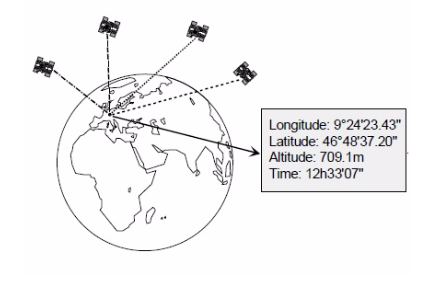
\includegraphics[width=10cm]{img/theory/GPS/gps_introduction.png}
	\caption{Model działania systemu GPS. Źródło: \cite{GPS_ublox}}
	\label{fig:image_gps_basics}
\end{figure}

Podstawę w systemach GNSS stanowi czas. Każdy z satelitów posiada 4 zegary atomowe, które stanowią najdokładniejsze źródło czasu znane ludzkości. Zegary te posiadają błąd rzędu 1 sekundy po upływie najwcześniej 30000 lat. Dodatkowo, są one co pewien czas synchronizowane ze źródłami na Ziemi.

Zadaniem każdego z satelitów jest nadawanie w formie rozgłoszeniowej sygnału, w którym zawarta jest wiadomość o jego lokalizacji na orbicie oraz czasie w momencie wysyłania wiadomości. Sygnał ten nadawany jest drogą radiową więc jego prędkość jest równa prędkości światła. Po dotarciu do odbiornika jest on bardzo słaby, przez co praktycznie niemożliwe jest jego odebranie wewnątrz budynków, a w pobliżu wysokich obiektów dokładność lokalizacji spada. Najdokładniejsze wyniki wyznaczania pozycji można osiągnąć na otwartej przestrzeni. Podstawowy sygnał przesyłany jest na fali nośnej o częstotliwości 1575.42 MHz i nosi nazwę L1.

Ponadto, sygnał GPS (a także pochodzący z innych systemów lokalizacji satelitarnej) ulega łatwo zakłóceniom w momencie przejścia przez jonosferę, bowiem fala elektromagnetyczna ulega na niej załamaniu, przez co zmienia swój tor i wydłuża drogę. W efekcie, pomiary odległości od odbiornika do satelity, niezbędne do wyznaczenia lokalizacji przestają być dokładne i pojawia się błąd lokalizacji.
Problem ten rozwiązano na 2 sposoby. Pierwszym z nich jest nadawanie sygnału przez satelity na kilku częstotliwościach. Każda z nich, przechodząc przez jonosferę ulega załamaniu, lecz pod innym kątem, przez co pokonają różne długości drogi przebytej do odbiornika, a tym samym zostaną odebrane w różnych momentach. Dzięki temu, odbiornik jest w stanie wyznaczyć korektę i wyeliminować błąd. Pierwotnie, rozwiązanie to było dostępne jedynie w celach militarnych, lecz od 2005 roku, Departament Obrony Stanów Zjednoczonych udostępnił częstotliwość L2 (1227.60 MHz) do celów cywilnych, a od 2008r. - również L5 (1176.45 MHz). Częstotliwości dostępne w systemie GPS pokazano na rysunku \ref{fig:image_gps_frequencies}.

\begin{figure}[H]
	\centering
	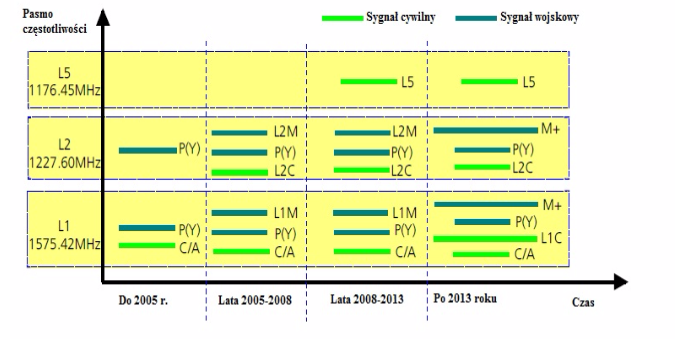
\includegraphics[width=15cm]{img/theory/GPS/gps_frequencies.png}
	\caption{Zbiór częstotliwości wykorzystywanych w systemie GPS. Źródło: \cite{inzynierka}}
	\label{fig:image_gps_frequencies}
\end{figure}

Druga metoda to wyznaczenie korekty dla przejścia przez jonosferę w stacjach naziemnych, a następnie rozgłaszanie depeszy ją zawierającej poprzez sieć stacji bazowych. Rozwiązanie to nosi miano DGPS (\textit{ang. \textbf{D}ifferential \textbf{GPS}}). Dzięki zastosowaniu tej techniki, dokładność lokalizacji wzrasta z nominalnych 15 m nawet do 10 cm.

Układy GPS, które umożliwiają skorzystanie z któregoś z tych dwóch rozwiązań są jednak kosztowne, więc na rynku cywilnym najpowszechniej stosowane są moduły wykorzysujące jedynie częstotliwość L1. Dzięki temu, za kilkadziesiąt złotych można uzyskać system z dokładnością do kilku metrów w sprzyjających warunkach \cite{inzynierka} (Rozdział 7 - Testy urządzenia). W pracy tej uzyskano dokładność systemu rzędu 1 - 2 metrów przy braku zakłóceń, oraz 5 - 7 metrów idąc wzdłuż wysokich budynków.

Aby zrozumieć zasadę działania systemu GPS proszę wyobrazić sobie sytuację jak na rysunku \ref{fig:image_gps_basics1}:

\begin{figure}[H]
	\centering
	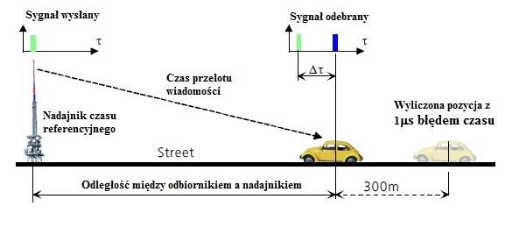
\includegraphics[width=12cm]{img/theory/GPS/gps_basics1.png}
	\caption{Zasada działania systemu GPS. Źródło: \cite{inzynierka}}
	\label{fig:image_gps_basics1}
\end{figure}

Załóżmy, że w przedstawionym pojeździe znajduje się odbiornik GPS. W pewnym momencie odbiera on sygnał GPS z nadajnika referencyjnego. W sygnale znajduje się wartość czasu w momencie wysłania wiadomości. Ze względu na skończoną prędkość światła ($c = 299 792 458 m/s$), zostanie ona odebrana przez odbiornik z pewnym opóźnieniem. Wykorzystując ten fakt i znając prędkość transmisji (wartość prędkości światła), można wyznaczyć odległość do nadajnika:

\begin{equation}
	D = c \cdot \Delta t
\end{equation}

gdzie,

$D$ - odległość między nadajnikiem i odbiornikiem

$c$ - prędkość światła

$\Delta t$ - różnica czasu między wysłaniem i odebraniem wiadomości

Aby wyznaczyć różnicę czasu, odbiornik powinien mieć również własny zegar. Powinien on być przy tym niezwykle dokładny i zsynchronizowany z zegarem w nadajniku, bowiem błąd rzędu 1 $\mu s$ powoduje błąd lokalizacji rzędu 300 m. Ponieważ uzyskanie takiej dokładności oraz synchronizacji w każdym odbiorniku jest niemożliwe, należało znaleźć sposób umożliwiający rezygnację z konieczności posiadania zegara w odbiorniku. Przedstawiono go na rysunku \ref{fig:image_gps_basics2}:

\begin{figure}[H]
	\centering
	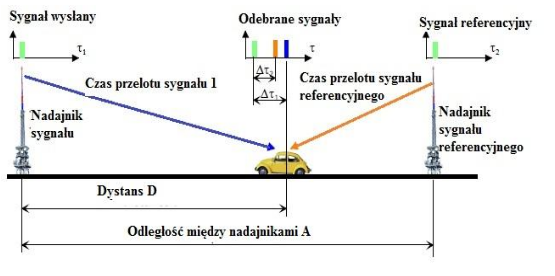
\includegraphics[width=12cm]{img/theory/GPS/gps_basics2.png}
	\caption{Zasada działania systemu GPS - sygnał referencyjny. Źródło: \cite{inzynierka}}
	\label{fig:image_gps_basics2}
\end{figure}

Polega on na zastosowaniu dodatkowego sygnału referencyjnego czasu. Wówczas po odebraniu obu sygnałów (które zostały wysłane w tym samym momencie) otrzymujemy:

\begin{equation}
\begin{cases}
\Delta \tau_1 \cdot c = D \\ 
\Delta \tau_2 \cdot c = A - D
\end{cases}
\end{equation}

Gdzie:

$\tau_1$ - różnica czasu między wysłaniem sygnału z nadajnika, a momentem jego odebrania

$\tau_2$ - różnica czasu między wysłaniem sygnału z nadajnika referencyjnego, a momentem jego odebrania

$A$ - odległość między nadajnikami

$D$ - odległość od nadajnika do odbiornika\\

Po odjęciu od pierwszego równania drugiego otrzymamy:

\begin{gather}
(\Delta \tau_1  - \Delta \tau_1) \cdot c = 2D - A \\
D = \frac{(\Delta \tau_1  - \Delta \tau_1) \cdot c + A}{2} \nonumber 
\end{gather}

Ponieważ jednak:

\begin{equation}
\begin{cases}
	\Delta \tau_1 = t - \tau_1 \\
	\Delta \tau_2 = t- \tau_2
\end{cases}
\end{equation}

to

\begin{equation}
(\Delta \tau_1 - \Delta \tau_2) = ((t - \tau_1) - (t - \tau_2)) = \tau_2 - \tau_1
\end{equation}

Gdzie:

$t$ - czas w momencie nadania sygnału przez nadajniki

$\tau_1$ - różnica czasu między wysłaniem sygnału z nadajnika, a momentem jego odebrania

$\tau_2$ - różnica czasu między wysłaniem sygnału z nadajnika referencyjnego, a momentem jego odebrania

Powyższe równania prowadzą do wniosku, że zastosowanie dodatkowego nadajnika referencyjnego, zsynchronizowanego z satelitami powoduje eliminację konieczności posiadania zegara w odbiorniku.

W rzeczywistości, takim nadajnikiem referencyjnym jest inny satelita GPS, bowiem są one ze sobą zsynchronizowane i nadają w dokładnie tym samym momencie.

Wyznaczona powyżej odległość $D$ dotyczy odcinka (jednej współrzędnej), a w rzeczywistości do wyznaczenia lokalizacji, uwzględniając satelitę referencyjnego, potrzeba sygnału z co najmniej 4 satelitów.

